\documentclass[12pt]{article}
%\documentclass[12pt, letterpaper, twoside]{article}
\usepackage{graphicx}
\usepackage{xcolor}
\usepackage{subcaption}
\usepackage{hyperref}
\definecolor{linkcolour}{rgb}{0,0,1}
\hypersetup{colorlinks=true, urlcolor=linkcolour, linkcolor=linkcolour, linkbordercolor=linkcolour, pdfborderstyle={/S/U/W 1}} 
\urlstyle{same}

\usepackage{setspace} 
\singlespacing

\usepackage{geometry}
\geometry{margin=0.5in}

\setlength\parindent{0pt}

\graphicspath{{images/}}

\begin{document}
\title{Bike-Share Case Study}
\date{}
\maketitle

This report provides the step-by-step explannation of the data analysis performed for a bike-sharing case study. The data belongs to a company that has two kinds of users: annual members and casual riders. The aim of the marketing team target is to convert casual riders into annual members in the next campaign. Thus, the goal of the study was to identify how annual members and casual riders use the bikes differently in order to provide the marketing team with insights. The data on which the analysis was carried out is from January-December 2023 and was downloaded from \href{https://divvy-tripdata.s3.amazonaws.com/index.html}{here}. \\

The library Pandas from Python was used to perform the analysis, and Matplotlib was used to plot the results. The code can be found in the Jupyter Notebook \href{https://github.com/SummerKassem/BikeShareCS/blob/main/PythonCode/bike_share_analysis.html}{here}. \\

This report consists of the following sections:
\begin{enumerate}
	\item Importing
	\item Exploration
	\item Cleaning
	\item Preparation
	\item Analysis
	\item Conclusion
\end{enumerate}

\section{Importing:}

\begin{itemize}
	\item reading the data:\\
	This method reads the bike rides from each .csv file (month), stores each month into a DataFrame (DF), and then concatenates the data into a single multi-index DF. Using a multi-index DF allows the distinction between the different months to still be maintained, while also facilitating the aggregation of values across the entire year when needed. In Figure (\ref{fig1}) we can see the first and last 5 entries of bike rides from the concatenated multi-index DF:

	\begin{figure}[h]
	\hspace{-1.1cm}
	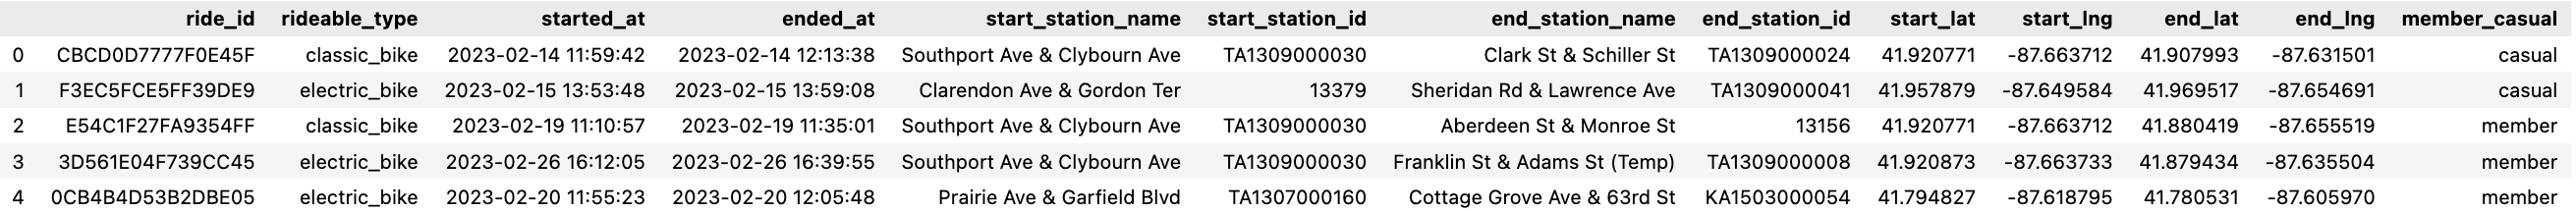
\includegraphics[scale=0.45]{img1.png}
	\caption{First and last 5 entries of bike rides from the original data}
	\label{fig1}
	\end{figure}
	\pagebreak
	
	In Figure (\ref{fig1}) the multi-index of the DF is shown in the first two columns (month, row\_id). Then looking at the entries themselves we can see that the data consists of 13 columns: 1) ride id, 2) type of bike, 3-4) date and time for the start and end of the ride, 5-12) the name, id, latitude and longitude of the start and end stations, and 13) whether the rider was a casual rider or a member.  \\
	
	\item \textit{count\_entries}:\\
	This method shows the number of bike rides in each month, the total number of bike rides in the dataset (year 2023), and the average per month. The result is shown in Figure (\ref{fig3_1}). The dataset contains in total almost 5.7 Million entries, with an average of approximately 480,000 rides per month. From Decemeber to March the number of rides is relatively lower than the average, which is expected as these are cold months. This is confirmed by the peak highlighted in August. After retrieving this information for the original dataset, the duplicates are dropped, and the method is called again. The result of running the method after dropping the duplicates is shown in Figure (\ref{fig3_2}). The number of entries before and after is identical, therefore the original dataset did not have any duplicates.\\ 
	
	\begin{figure}[h]
	\centering
	\begin{subfigure}{.4\textwidth}
	\hspace{0.5 in}
		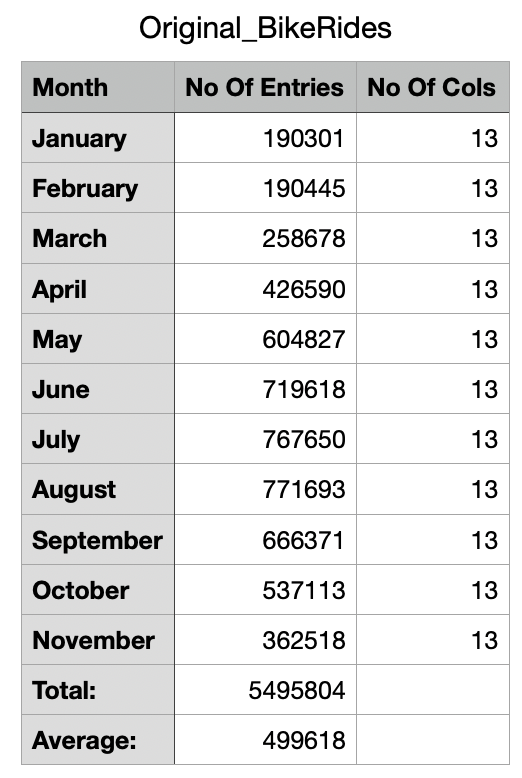
\includegraphics[scale=0.5]{img2.png}
		\caption{}
		\label{fig3_1}
	\end{subfigure}
	\begin{subfigure}{.4\textwidth}
	\hspace{0.5 in}
		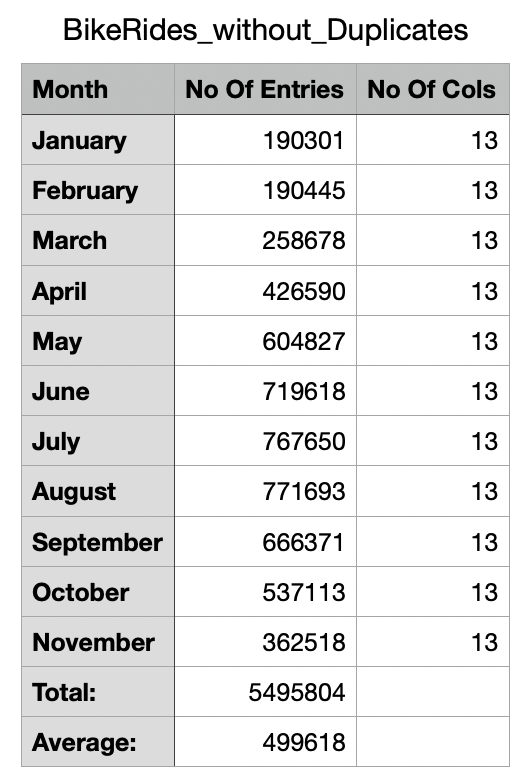
\includegraphics[scale=0.5]{img3.png}
		\caption{}
		\label{fig3_2}
	\end{subfigure}
	\caption{Total no of entries and average over the year, before and after removing duplicates}
	\label{fig3}
	\end{figure}

	\item \textit{get\_null\_percentage}:\\
	This method calculates the percentage of null values for each column. The results are shown in Figure (\ref{fig4}). As we can see the columns \textit{start\_station\_name}, \textit{start\_station\_id}, \textit{end\_station\_name}, \textit{end\_station\_id} in every month have 13-17\% null values. The columns \textit{end\_lat} and \textit{end\_long} have less than 1\% null values. \\
	
	\begin{figure}[h]
	\hspace{-0.5in}
	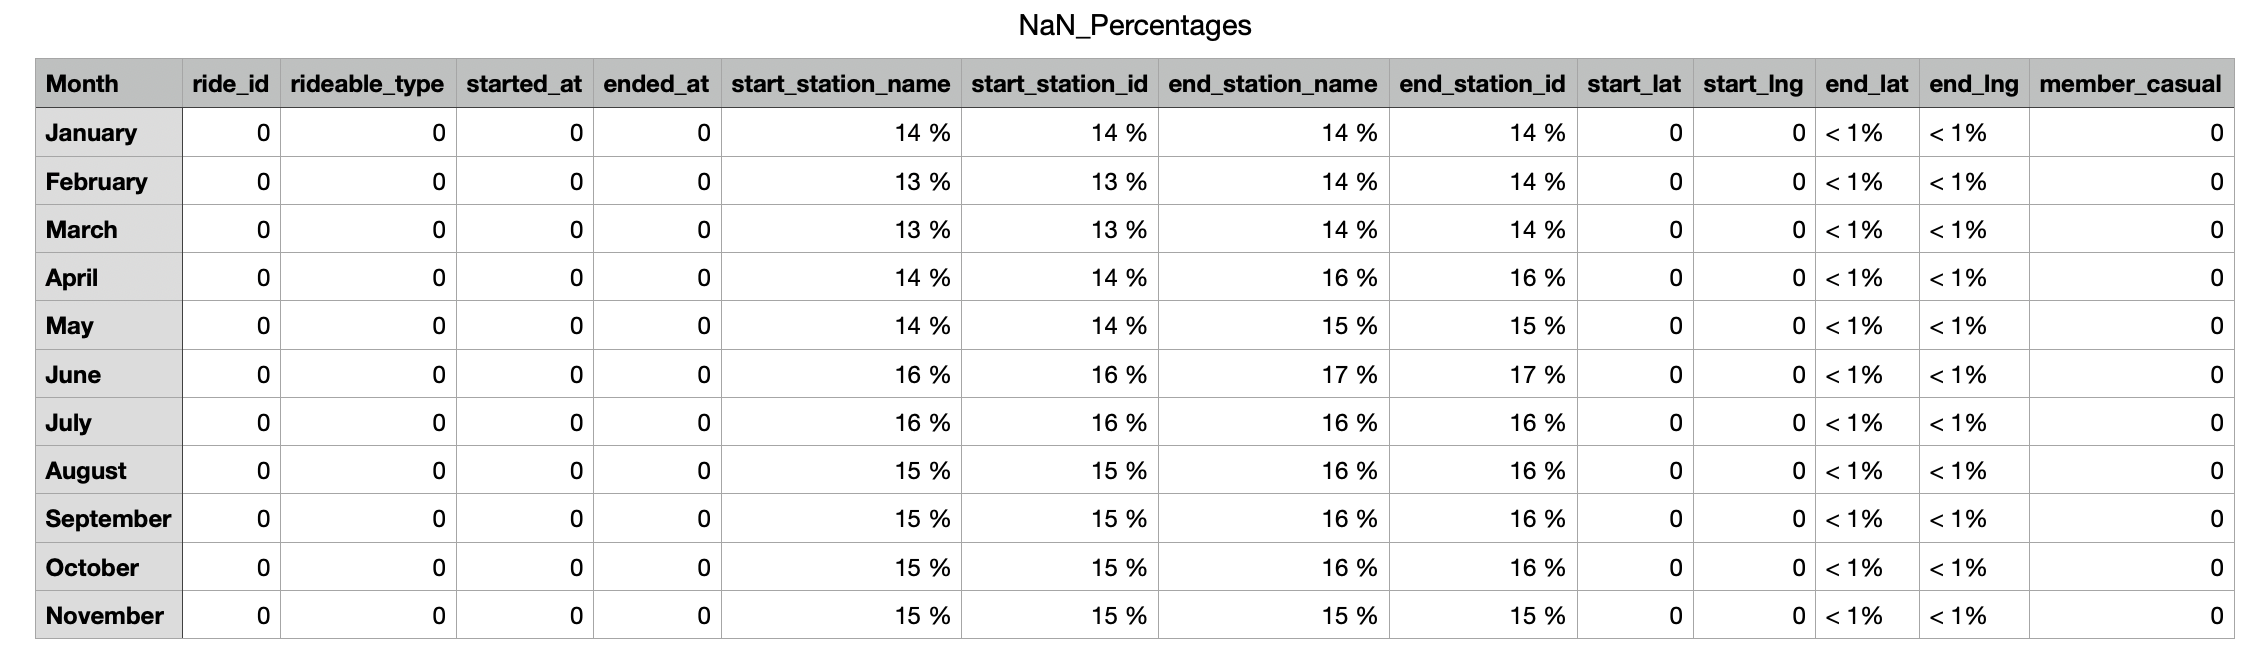
\includegraphics[scale=0.48]{imgNAN.png}
	\caption{Percentage of null values for each column}
	\label{fig4}
	\end{figure}
	
	\item \textit{get\_unique}:\\
	This method gets the number of unique (distinct) values for each column in the month of May. The result is shown in Figure (\ref{fig2}). The choice of the month of May is random and should not make a difference. 
	
	\begin{figure}[h]
	\centering
	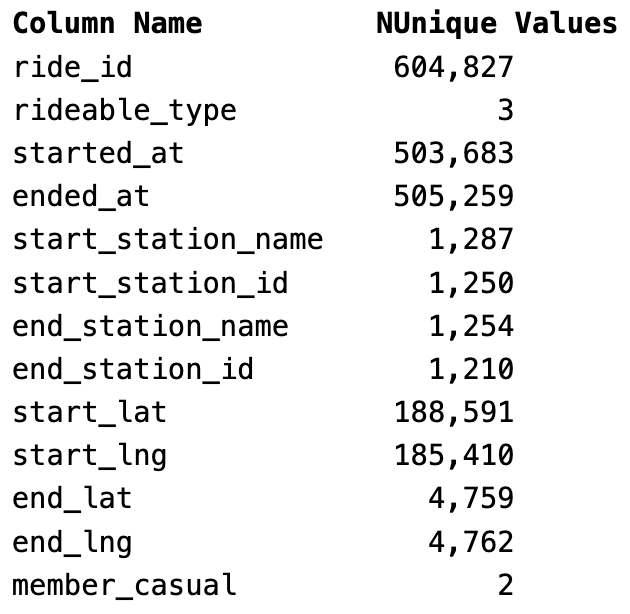
\includegraphics[scale = 0.6]{imgUni.png} 
	\caption{No. of unique values for every column for the month of May}
	\label{fig2}
	\end{figure}
	
	\begin{itemize}
	\item \textit{ride\_id\_unique}  = 604,827: as expected, \textit{ride\_id} has as many unique values as the number of entries in the dataframe.
	\item \textit{rideable\_type\_unique} = 3: these 3 values are the types of bikes that are offered by the company, which are: \Big(electric\_bike, classic\_bike, docked\_bike\Big).
	\item \textit{started(ended)\_at\_unique} = 503,683,  505,259: since these are datetimes (yy-mm-dd hh:mm:ss), one may have expected them to have as many distinct values as the \textit{ride\_id\_unique} = 604,827. Because, at a first glance, it seems unlikely for more than one rider to have rented a bike at the exact same time as another rides down to the second. However, the number of unique values in these columns is less than the number of entries by 16\%. Which means that 16\% of the bikes rides have the same \textit{started\_at} as other rides. To explore this a bit further, one of these duplicates has been retrieved and is shown in Figure (\ref{fig10}). By looking at the rides, it is clear that they are indeed different entries but with the exact same start time. \\
	
	\begin{figure}[h]
	\hspace{-0.5in}
	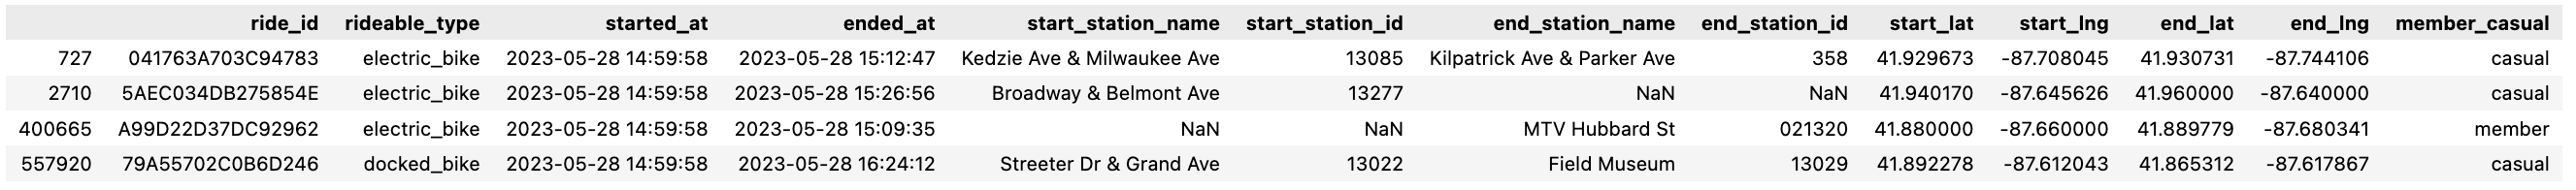
\includegraphics[scale=0.46]{imgDups1.png}
	\caption{Entries from May that have the same \textit{started\_at} date and time}
	\label{fig10}
	\end{figure}
	
	\item \textit{start(end)\_station\_name(id)\_unique} = 1287, 1250, 1254, 1210: since there is a limited number of stations, it is expected that these columns have a smaller number of unique values than the number of entries. However, one would have expected the number of station names and ids to be the same, whereas the ids are less than the names by a small fraction. Which could either by accounted for by the null values (Fig. \ref{fig2}) or could mean that there are stations that have the different names but the same id.
	\item \textit{start(end)\_lat(long)\_unique} = 188,591, 185,419, 4759, 4762: the start latitude and longitude numbers seem to be as expected, which is less than the total number of entries, but more than the number of stations (this is based on the assumption that the exact location where a bike is parked can vary within the station especially that the values are given to the $6^{th}$ decimal place). However, there is a large difference between the number of values in the start ($\sim$188,000) and the numbers in the end ($\sim$4800). This difference cannot be accounted for by the null values in the end columns, since these were less than 1\%. If these values are true, that would mean that users rode there bikes from many start locations, but mostly ended up in a much smaller set of locations. Which cannot be the case since that would have been reflected in a similar difference between the number of start and end stations. 
	\item \textit{member\_casual\_unique} = 2: these 2 values are the types of riders, which are: \Big(member, casual\Big).
	\end{itemize}
\end{itemize}
	
\section*{Cleaning:}
After exploring the dataset, we can see that the extractable information can be divided into information about the:
	\begin{enumerate} 
	\item rider (casual/member)
	\item bike (electric/classic/docked)
	\item ride (start-end: time, date, location)
	\end{enumerate}
	
Since, the goal of the analysis is to find out whether to target converting casual riders into members or not, it seems that all the information is relevant to the analysis, with the exception of the ride location. This is based on the assumption that the amount paid by the rider is based on how long the bike was rented, regardless of where. Furthermore, the geographical location would have been important if for example the goal of the analysis was to find out whether more stations should be added and where to do so. Therefore, since the locations seem to be irrelevant, contain null values and discrepancies, these columns will be dropped in the cleaning process. The column \textit{ride\_id} also does not provide any valuable information for the current analysis. \\

Another task to be performed in the cleaning phase is data formatting. We have already looked at the columns \textit{rideable\_type} and \textit{member\_casual}, and ensured that they have only the expected values and no nulls. As for the columns \textit{started\_at} and \textit{ended\_at}, these do not have null values, but still need to be checked to ensure that the \textit{ended\_at} time always comes after \textit{started\_at} time. In order to compare the values in these columns, they first need to converted from strings of characters to a numerical date-time format. \\

\begin{itemize}
	\item \textit{drop\_and\_change\_format}:\\
	  This method performs three tasks. First, it drops all the columns related to geographical location and ride id. Second, it converts the columns \textit{started\_at} and \textit{ended\_at} from strings of characters to a numerical datetime format. Finally, the method returns a Series of flags which indicate whether or not the \textit{ended\_at} time is before the \textit{started\_at} time. 
	  
	  \item \textit{clean\_data}:\\
	  By using the flags returned by the method \textit{drop\_and\_change\_format}, the rides where \textit{ended\_at} time is before the \textit{started\_at} time can be filtered out as shown in Figure (\ref{fig8}). Looking at these entries, we can see that there are cases when the \textit{ended\_at} time is before the \textit{started\_at} time by just a seconds. It can be that in these incidents the start and end time were switched due to some glitch, perhaps the bike rental time being very short (shorter than the server response time). But there are also cases when the time difference is a few minutes. In the entire dataset of approximately 5.7 Million entries, there is a total of 272 entries that have this issue. Since, the dataset is large, the method \textit{clean\_data} simply drops these entries. \\

	\begin{figure}[h]
	\centering
	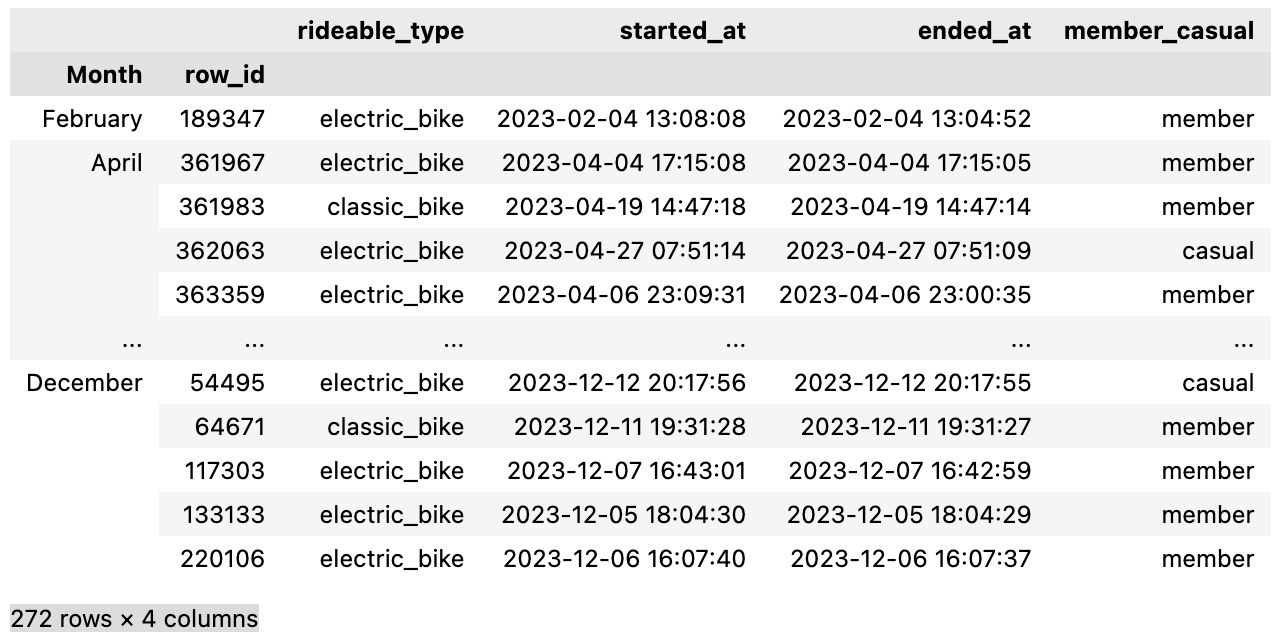
\includegraphics[scale=0.6]{imgNEG.png}
	\caption{Entries where the ended\_at time is before the started\_at time}
	\label{fig8}
	\end{figure}
	
	\end{itemize}
	
\section*{Preparation:}
Now that the dataset has been explored and cleaned, the next step is to prepare the data needed for analysis. Based on the assumption that the rides are charged according to how long they were rented, a column \textit{ride\_length} is added. Another column \textit{day\_of\_week} is also added to explore the behaviour of different riders a bit further. 

\begin{itemize}
	\item \textit{prepare\_data}:\\
	This method adds the two new columns: \textit{ride\_length}: the difference between the columns \textit{ended\_at} and \textit{started\_at} times, and \textit{day\_of\_week}: extracted from the date in \textit{started\_at}. The method then drops the columns \textit{started\_at} and \textit{ended\_at}, since the new columns make them redundant.
	
\end{itemize}

\section*{Analysis:}
Finally, the data can be analysed in order to determine how casual riders and members differ.

 \begin{itemize}
	\item \textit{count\_rides\_per\_rider}:\\
	This method produces a pivot table whose index is the month, and the columns are the number of rides for each rider type. The method also returns the total number of rides for the entire year. The resulting pivot table is shown in Figure (\ref{fig17_1}), and is visualised using the plot shown on the right Figure (\ref{fig17_2}). From the plot we observe that, per month there is approximately 100,000 more rides by members than by casual riders. Next, we see that rides by members and casual riders follow the same pattern of peaking during the summer months, and dropping during the winter months. 

	\begin{figure}[h]
	\hspace{0.8in}
	\begin{subfigure}{.2\textwidth}
		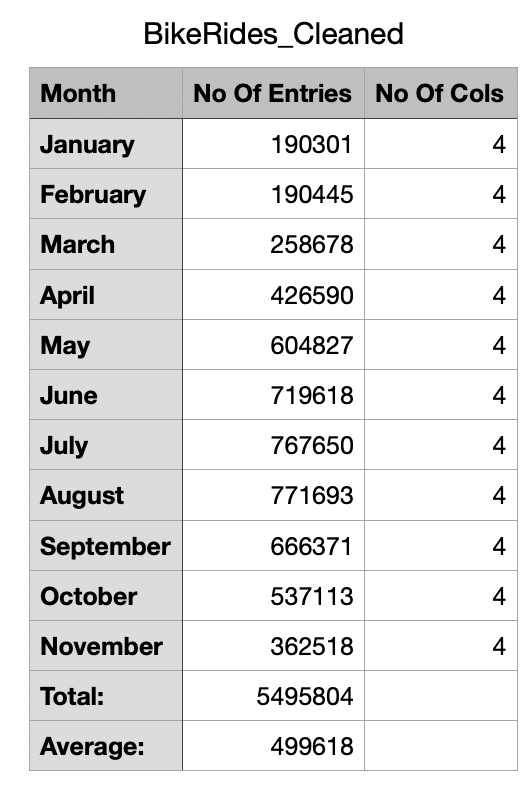
\includegraphics[scale=0.55]{img4.png} 
		\caption{}
		\label{fig17_1}
	\end{subfigure}
	\begin{subfigure}{.55\textwidth}
	\hspace{1.2in}
		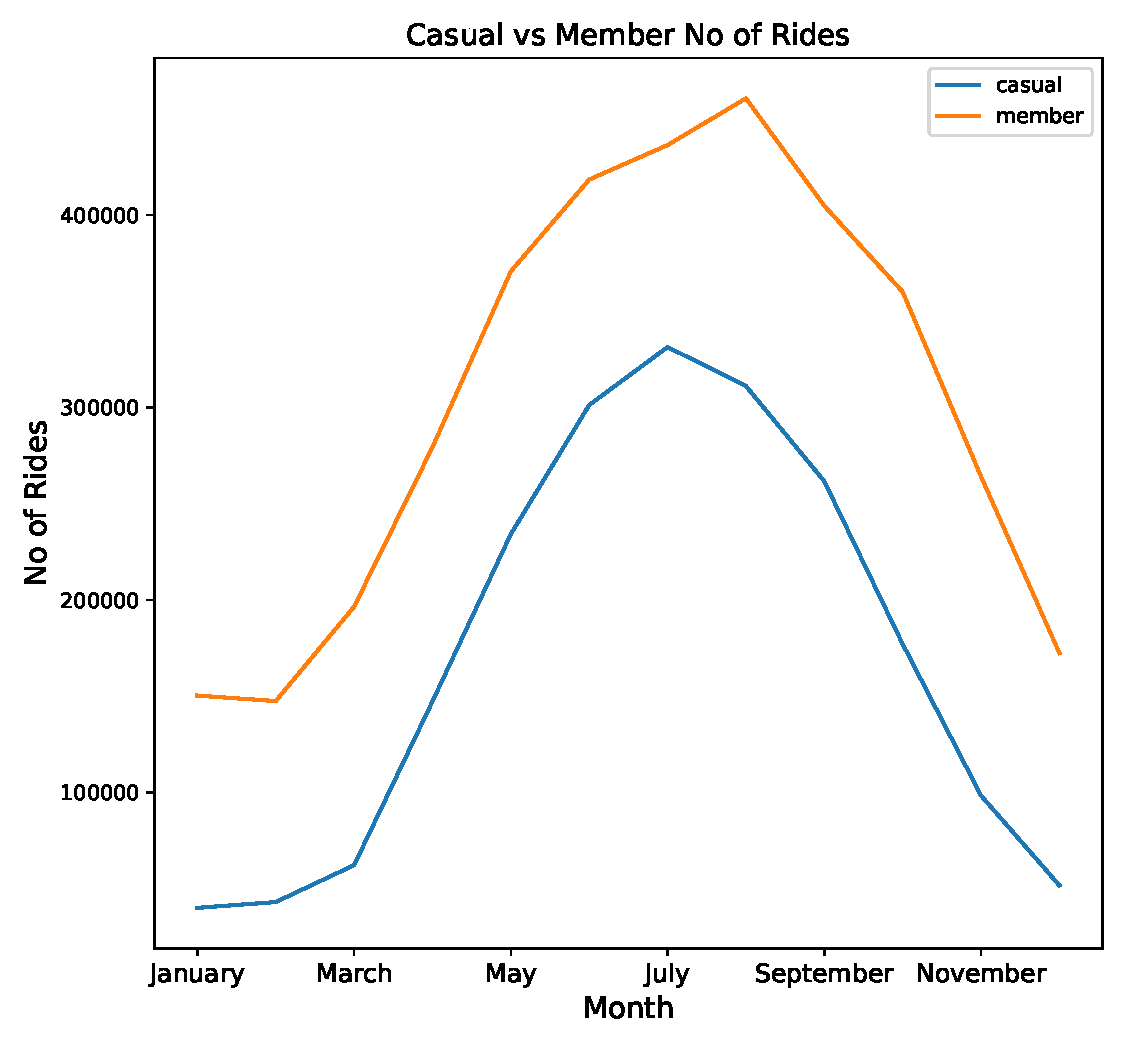
\includegraphics[scale=0.48]{no_of_rides.pdf}
		\caption{}
		\label{fig17_2}
	\end{subfigure}
	\caption{Total no of rides per rider type}
	\end{figure}
	
\item \textit{mean\_max\_by\_month}:\\	
	This method produces a pivot table whose index is the month, and the columns are the mean and maximum ride length for each rider type. The method also calculates the mean and max values across the entire year. The pivot table is shown in Figure (\ref{fig11_1}), and the corresponding visualisations are shown below. From the plot of the mean values in Figure (\ref{fig11_2_1}) we observe that casual riders have longer rides, than members across the entire year. Also, the mean ride length for casual riders varies across the year from approximately 20 minutes in the colder months to a peak of 35 minutes in August. As for members, their mean ride length changes only from 10 to 13 minutes. When looking at the maximum ride length plot in Figure (\ref{fig11_2_2}) we see a similar pattern: casual riders have longer rides, and their maximum ride lengths changes from 1 day in the cold months to 68 days in August. As opposed to, members whom have a maximum ride length of 1 day all throughout the year.\\
	
However, it is important to note here that such longer rides, as seen in the maximum ride length plot, are outliers that occur quite rarely in the dataset. This can be seen when plotting the entire dataset distribution of ride lengths using a box plot as shown in Figure (\ref{fig13}).  
\pagebreak
	\begin{figure}[h]
	\centering
		\begin{subfigure}[b]{0.55\textwidth}
   			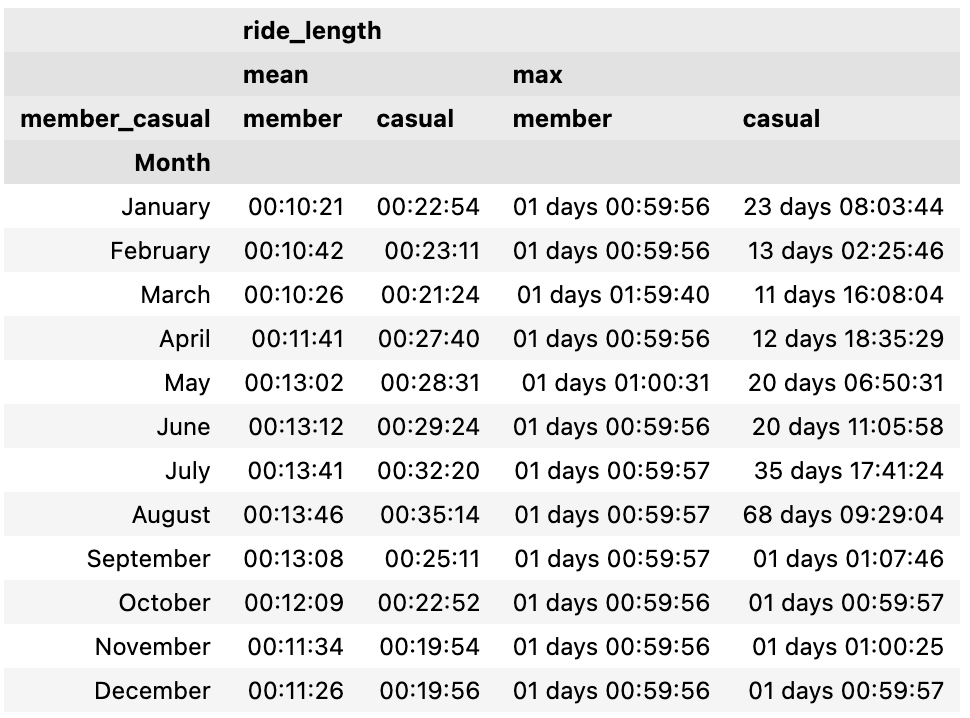
\includegraphics[scale=0.6]{imgMeanMax2.png} 
			\caption{}
			\label{fig11_1}
		\end{subfigure}

		\begin{subfigure}[b]{0.55\textwidth}
			\hspace{-1.5in}
   			\begin{subfigure}{.45\textwidth}
				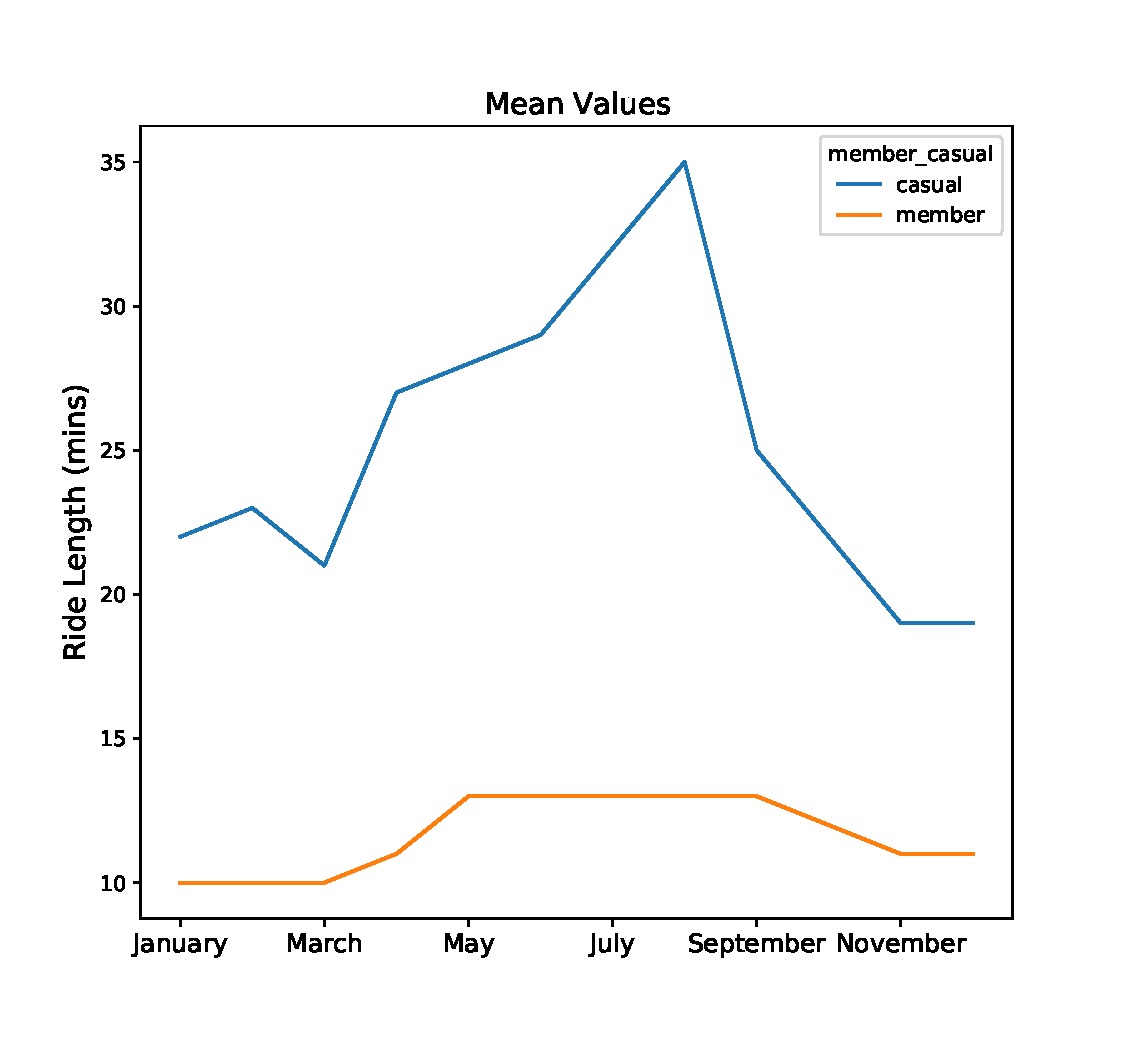
\includegraphics[scale=0.48]{mean_cvsm_month.pdf} 
				\caption{}
				\label{fig11_2_1}
			\end{subfigure}
			\hspace{1.5in}
			\begin{subfigure}{.4\textwidth}
				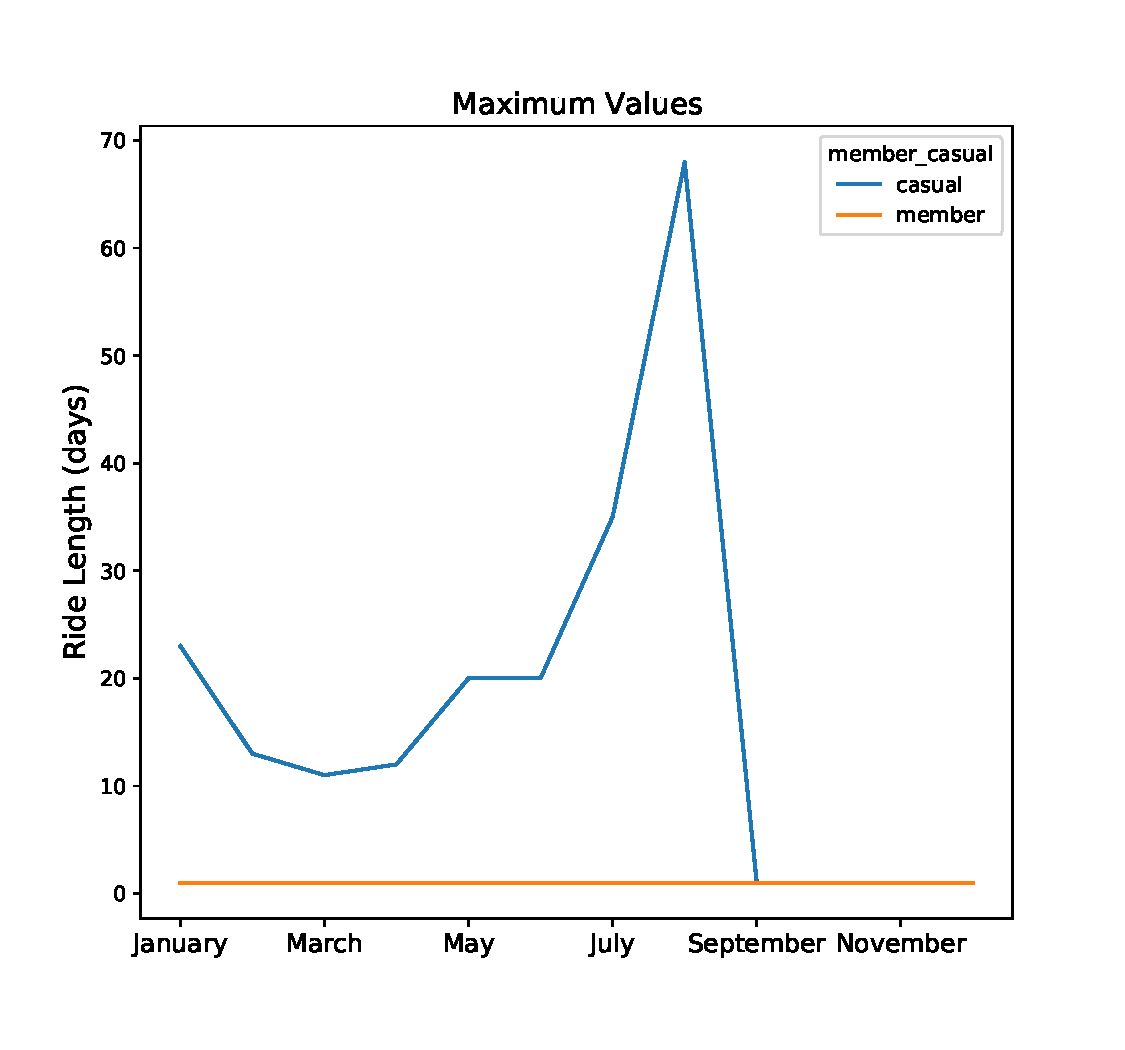
\includegraphics[scale=0.48]{max_cvsm.pdf}
				\caption{}
				\label{fig11_2_2}
			\end{subfigure}
		\end{subfigure}
		\caption{Mean and max ride length divided by rider type}
	\end{figure}
	

\pagebreak
	\begin{figure}[h]
	\centering
	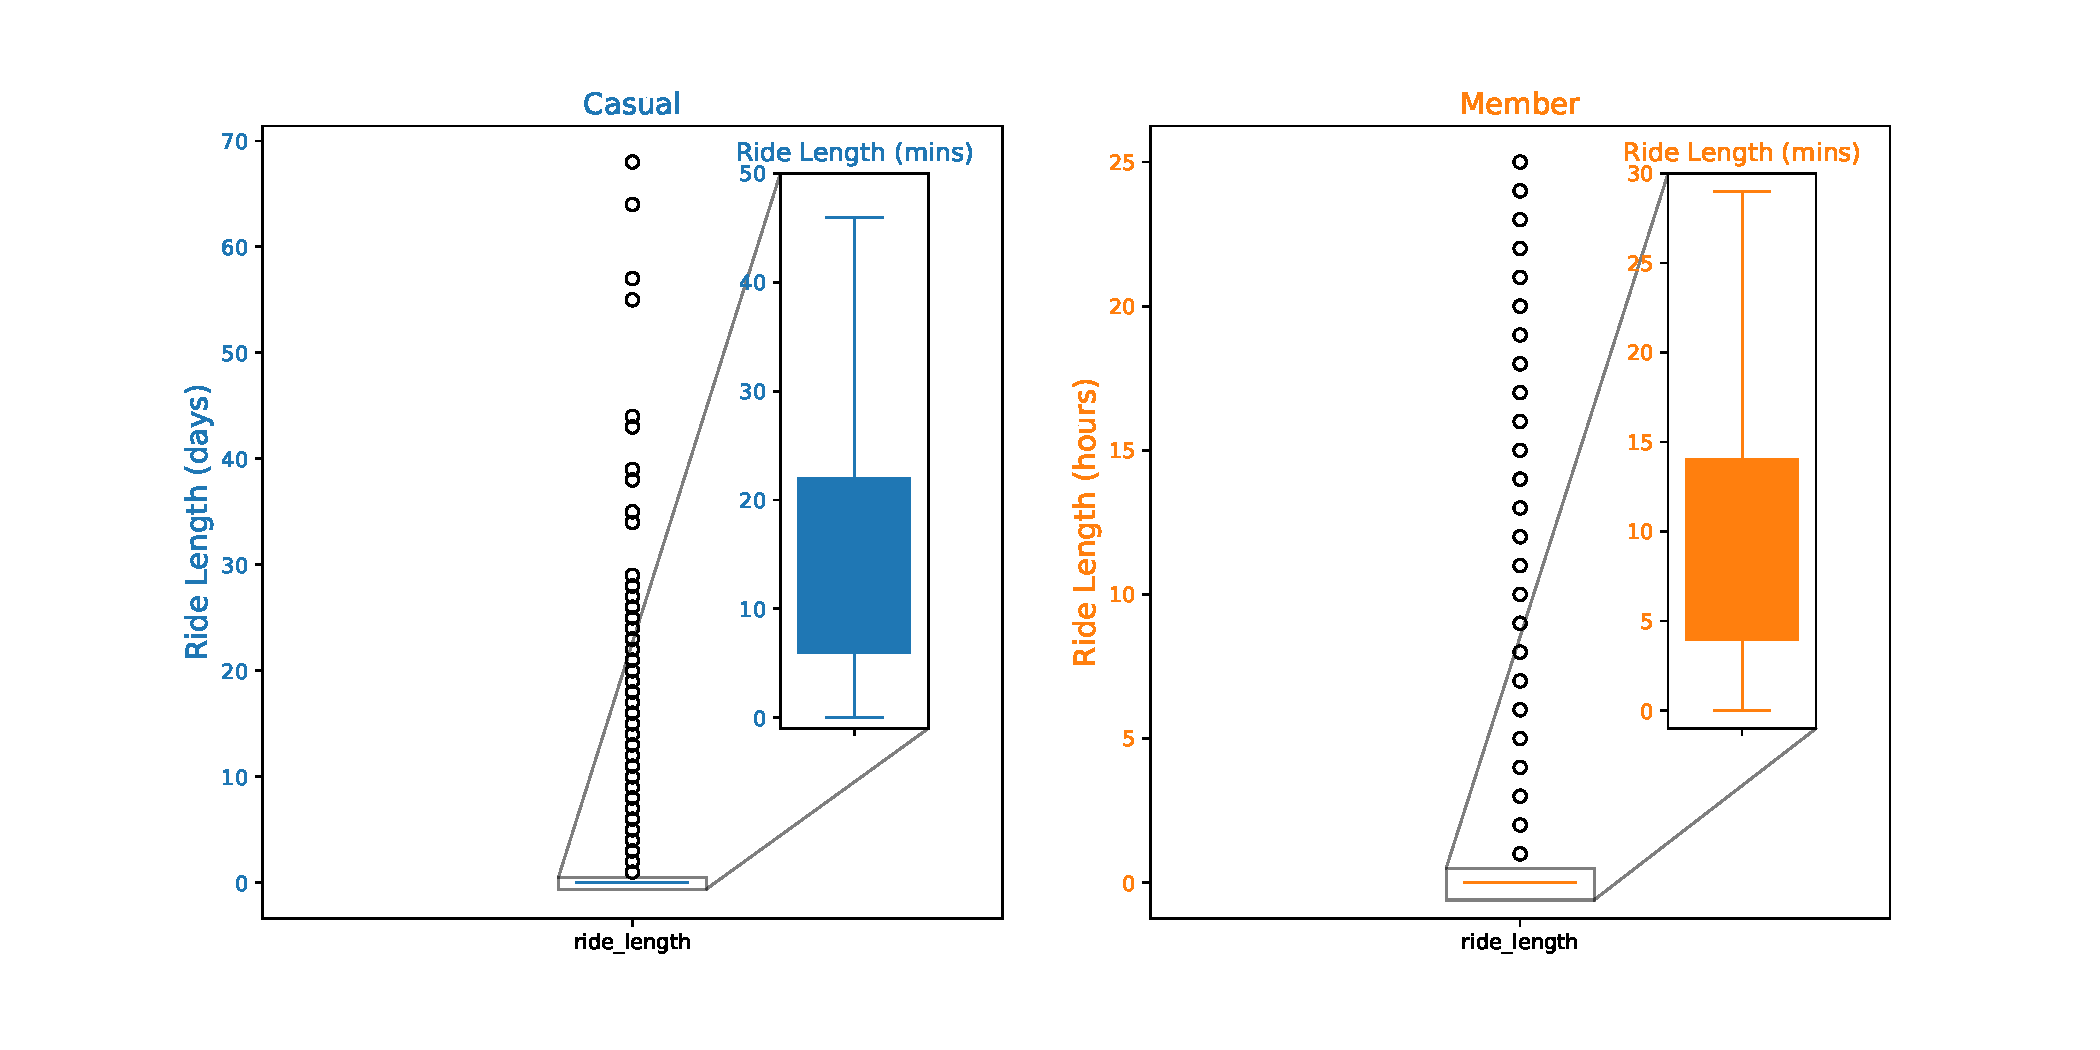
\includegraphics[scale=0.5]{boxplot_distribution.pdf} 
	\caption{Box plots of the distribution of values in the ride length for casual riders and members}
	\label{fig13}
	\end{figure}
	
A box plot typically divides the values in a distribution into 4 quartiles (0-25\%, 25-50\%, 50-75\%, 75-100\%), and displays them as follows: the middle 2 quartiles (25-75\% of the distribution) are shown inside a box, the lower and upper 25\% are shown by whiskers, and circles are used to represent outliers. From Figure \ref{fig13} (left) we can see that, for casual riders, the outlier points are the ones that occupy the range [1 - 70] days, whereas the distribution itself can only be seen in the [0 - 50] minute range. As for the members (Fig. (\ref{fig13}) right), the distribution of ride lengths is in the [0 - 30] minute range, and its outliers are in the [1- 25] hour range. Therefore, in order to see the comparison between the ride lengths for casual riders and members more clearly, the outliers are dropped, and the box plots, are shown side by side in Figure (\ref{fig15}). 

	\begin{figure}[h]
	\centering
	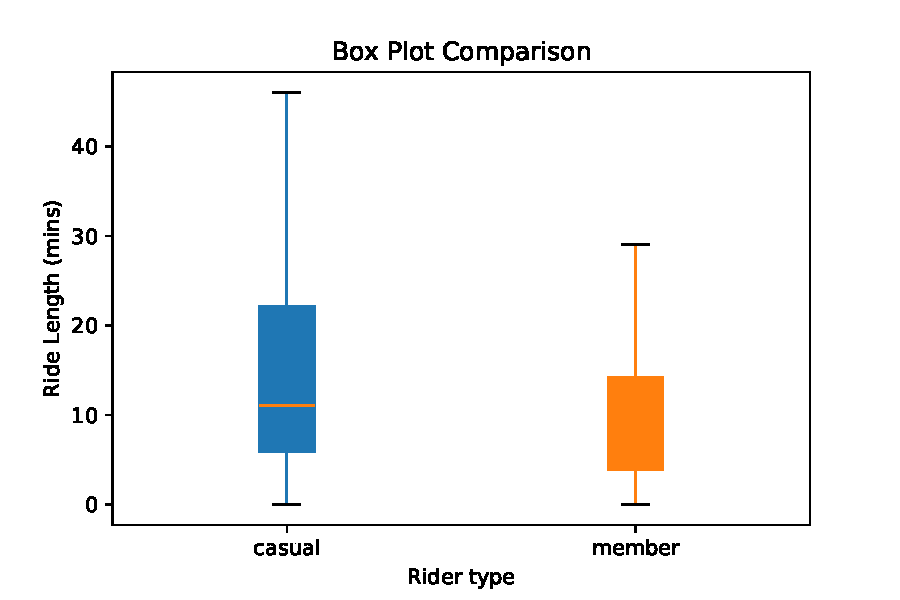
\includegraphics[scale=0.5]{boxplot_distribution2.pdf} 
	\caption{Box plot comparison between the ride lengths of casual and member riders without outliers}
	\label{fig15}
	\end{figure}
\pagebreak
Figure (\ref{fig15}) shows that the main distribution (i.e. without outliers) of ride lengths for casual riders varies between [0 - 46] minutes, and that the middle 50\% of the values are between [6 - 22] minutes. As opposed to members whose ride length vary between [0 - 29] minutes, and the middle 50\% are between [4 - 14] minutes. The mean values calculated from the entire distribution are marked on the plot using the green stars. For casual riders the mean is 27.7 minutes (slightly higher than the mean calculated first by month and then for the year = 25.7 Figure (\ref{fig11_1})), and for members it is 12 minutes.  
	
	\item \textit{mean\_by\_day\_of\_week:}\\
	So far we have compared the rider types either by first grouping the data using the month (Fig. \ref{fig11_2_1}) or by looking at the entire distribution (Fig. \ref{fig13}). In order to get a different perspective, we will now look at the mean value of the ride length after the data has been grouped by the day of the week. The resulting pivot table as well as its visualisation are shown in Figure (\ref{fig14}). Here we see the same higher average for the casual riders when compared to members, with a peak for casual riders during the weekend. 
	
	\begin{figure}[h]
	\hspace{0.8in}
	\begin{subfigure}{.2\textwidth}
		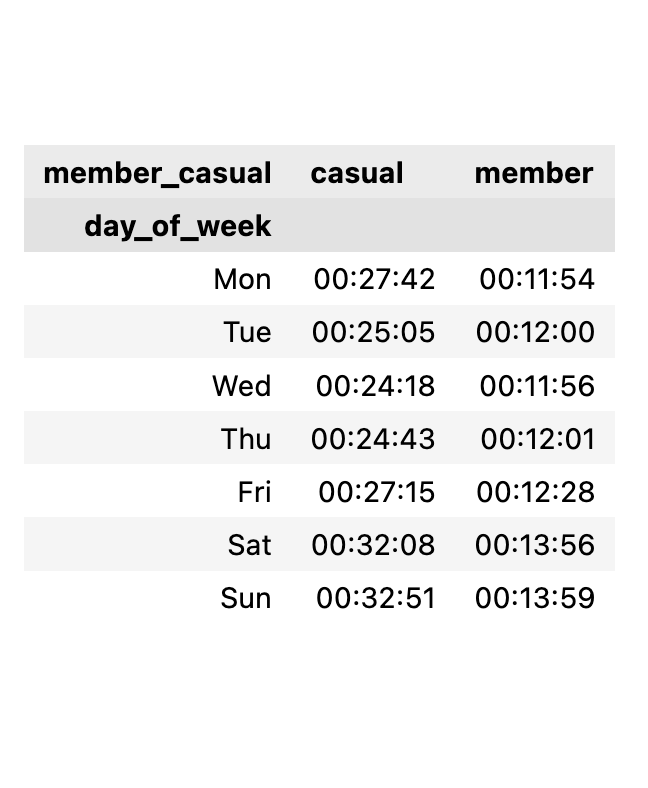
\includegraphics[scale=0.6]{dayofweek_t.png} 
		\caption{}
		\label{fig14_1}
	\end{subfigure}
	\begin{subfigure}{.55\textwidth}
	\hspace{1.2in}
		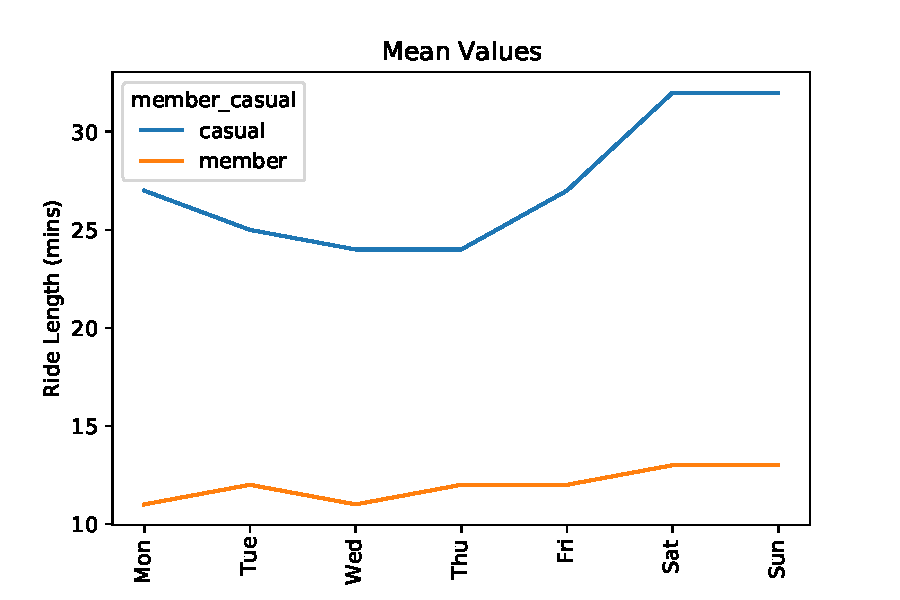
\includegraphics[scale=0.48]{mean_cvsm_dayofweek.pdf} 
		\caption{}
		\label{fig14_2}
	\end{subfigure}
	\caption{Mean ride length per rider type grouped by day of the week}
	\label{fig14}
	\end{figure}
	\pagebreak

	\item \textit{count\_rideable\_type}:\\
	This method produces a pivot table with the rider type (casual/member) as an index, and the columns are rideable type, which is the type of bike (classic/docked/electric). The values are the number of entries in each category. The result is visualised in Figure (\ref{fig16}). From the histogram we can see that for classic and electric bikes, there are more member rides than casual rides. Which is to be expected, since the overall number of member rides is larger than the casual riders (Fig. \ref{fig17_1}). However, the interesting finding is that when it comes to docked bikes, only casual riders have used those in 2023.
	
	\begin{figure}[h]
	\centering
	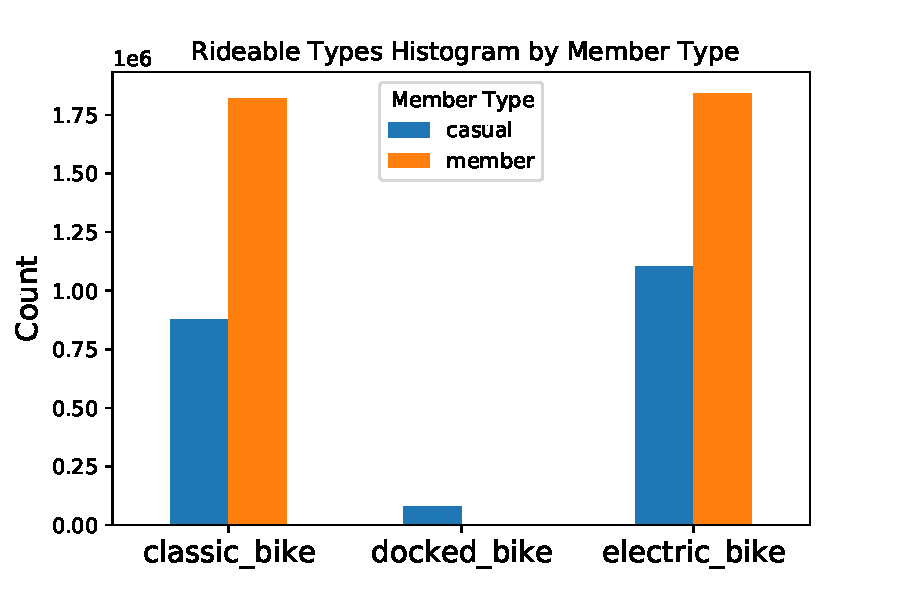
\includegraphics[scale=0.6]{rideable_types.pdf} 
	\caption{No of Rides for each type of bike per rider type}
	\label{fig16}
	\end{figure}
	
\end{itemize}

\pagebreak

\section*{Conclusion:}

In this report, the analysis of a bike-sharing case-study was presented. First, the dataset was explored by looking at   what the original data consisted of, what were the unique values in each column, as well as the percentage of null values. For the year 2023, on average, there were $\sim$480,000 rides per month. During the cold months December-March the rides dropped to $\sim$200,00, and in the summer months they went up to $\sim$770,000 rides. No duplicates were found in the dataset, but the columns \textit{start(end)\_station\_name(id)} had 13-17\% null values, and the columns \textit{end\_lat(long)} had less than 1\% null values. When looking at the number of unique values for each column, some discrepancies were found, for example there were more station names than there were station ids. Next, the data was cleaned by dropping the columns that had inconsistencies, null values or were irrelevant to the analysis. The data was also formatted by converting the start and end times into date-time numerical values and the entries where the end time was before the start were dropped. In order to prepare the data for analysis, the columns ride length and day of the week were added. \\

The data was then analysed by first looking at the number of rides performed by members versus casual riders. The entire dataset for the year 2023 consists of 5.7 Million rides, 64\% of which were made by members, and 36\% were by casual riders. The dataset was then grouped by month, and the average and maximum ride length were calculated per rider type. For members the mean ride length in 2023 was $\sim$12 minutes, whereas for casual riders it was $\sim$25 minutes. When looking at the maximum ride length it was shown that members never rented the bike for more than one day, whereas casual riders had a maximum ride length ranging from 1 - 68 days. However, by plotting the entire distribution of ride length values using box plots, it was shown that such longer rides were outliers that occurred quite rarely. The box plots showed that the main distribution of ride lengths after ignoring the outliers can be summarised by the values shown in Table (\ref{table1}): \\

\begin{table}[h]
\begin{center}
\begin{tabular}{ | c | c | c| c | c |  } 
\hline
   	& 0 - 25\% 	& 25 - 70\% 	& 75 - 100\% &  mean (mins)  \\ 
  \hline
casual 	& 0 - 6 		&  6 - 22 		& 22 - 46 & 27 \\
\hline
member 	& 0 - 4 		& 4 - 14		& 14 - 29 & 12 \\
\hline
\end{tabular}
\caption{Distribution of ride lengths (minutes) for casual riders and members without outliers}
\label{table1}
\end{center} 
\end{table}


By looking at the results shown in Table (\ref{table1}) we can confidently conclude that casual riders have longer ride lengths, whether we compare the mean across the whole dataset, or if we compare each quartile of the distribution. Therefore, this analysis supports the recommendation to target converting casual riders into members. Lastly, it was found that in the year 2023, docked bikes were used only by casual riders. So it might be beneficial to use that information within the marketing campaign.

\end{document}